\documentclass[a4paper]{article}



%% Sets page size and margins
\usepackage[a4paper,top=2cm,bottom=2cm,left=3cm,right=3cm,marginparwidth=1.75cm]{geometry}

%% Useful packages
\usepackage{amsmath,amsthm,amssymb,amsfonts,graphicx, fancyvrb}
\usepackage{drawstack}

\title{\vspace{-1.5cm}IERG4130 Lab 2 Report}

\author{LAU Long Ching\\SID: 1155127347\\
        
}

\date{12/04/2021}



\begin{document}
\maketitle
\section{TCP/IP Attack}
\subsection{Task 1: SYN Flooding Attack}
\subsubsection{Lab Setup}
I first created three VMs, namely Client (10.0.2.15), Server (10.0.2.4) and Attacker (10.0.2.5). They are connected to the same LAN following the guidelines.\\\\
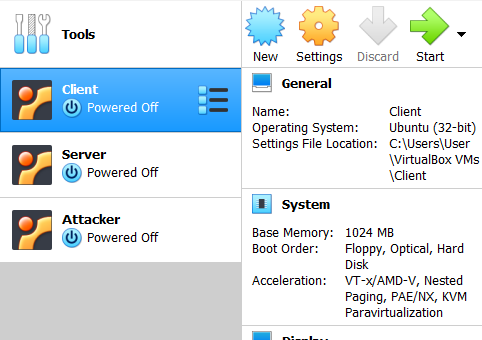
\includegraphics[scale=0.7]{1/1.png}\\\\
Here is the size of the queue:\\\\
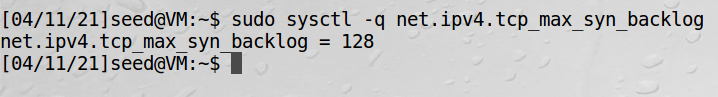
\includegraphics[scale=0.7]{1/2.png}\\\\
And we can check the usage of the queue using \verb+netstat -tna+:\\\\
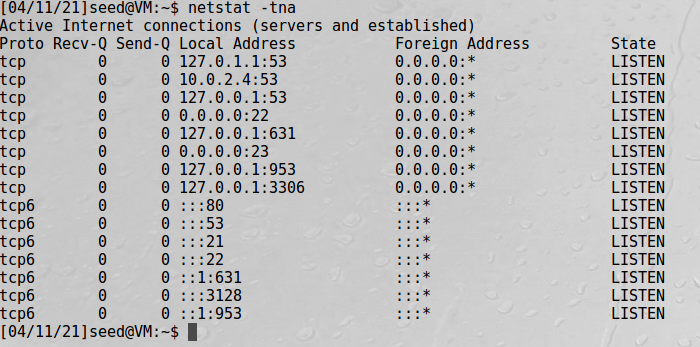
\includegraphics[scale=0.7]{1/3.png}\\\\
\pagebreak
\subsubsection{The Attack}
First we try connecting the client to the server, and we can see that it runs smoothly.\\\\
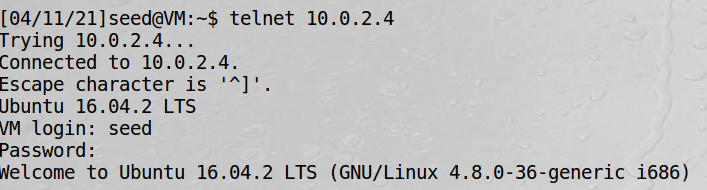
\includegraphics[scale=0.7]{1/4.png}\\\\
From the server VM, we can see that the connection is established.\\\\
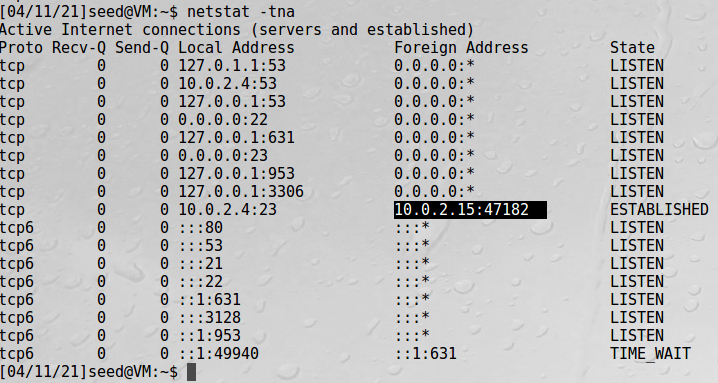
\includegraphics[scale=0.7]{1/5.png}\\\\
We now try to initiate an SYN flooding attack.\\\\
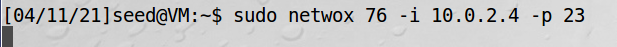
\includegraphics[scale=0.7]{1/6.png}\\\\
On the victim machine, we can see that \verb+netstat -tna+ result is spammed with connections with state as \verb+SYN-RECV+, indicating half-open connections.\\\\
\pagebreak
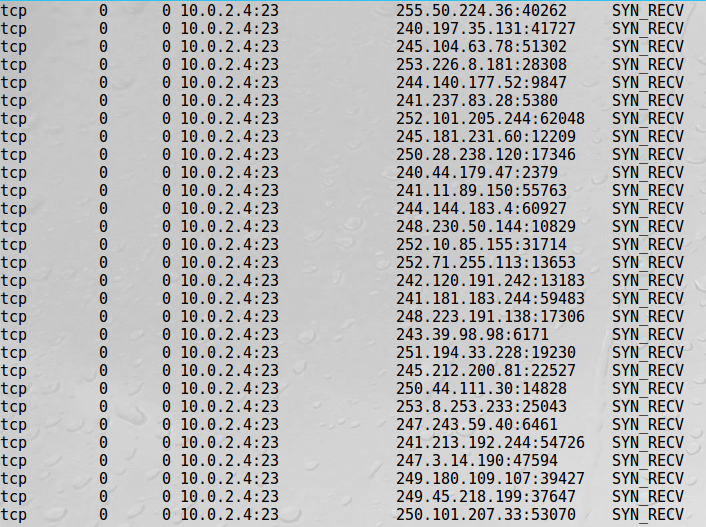
\includegraphics[scale=0.7]{1/7.png}
\\Using Wireshark, we can see a large flood of SYN connections. We see that the victim machine receives numerous numbers of connection on port 23 from random IP addresses spoofed by the \verb+netwox+. \\\\
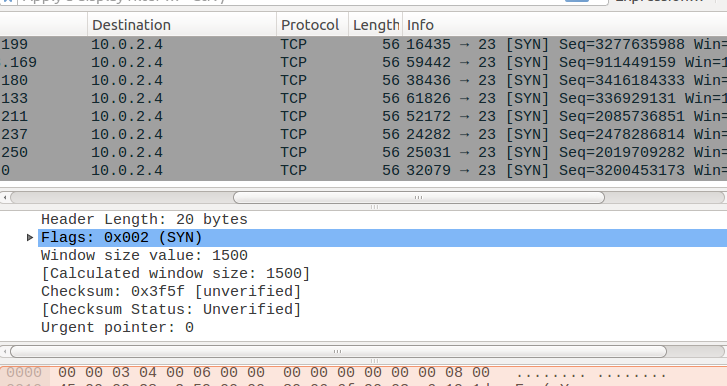
\includegraphics[scale=0.7]{1/7_1.png}\\\\
However, the attack seems unsuccessful, as the victim can still start a \verb+telnet+ connection to the server.\\\\
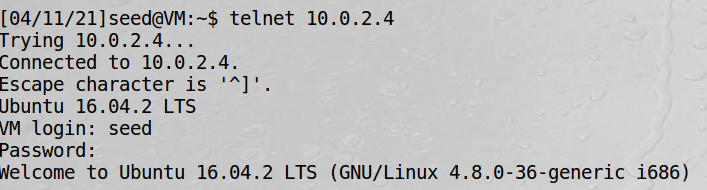
\includegraphics[scale=0.7]{1/4.png}\\\\
\subsubsection{SYN Cookie Countermeasure}
So now, we check if the SYN cookie is on, and indeed it is. So we turn it off.\\\\
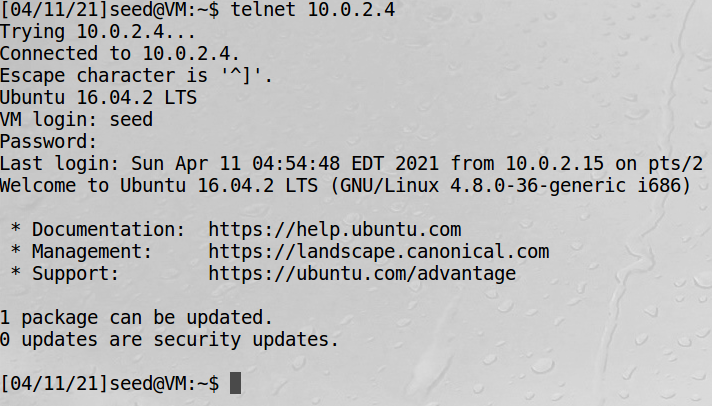
\includegraphics[scale=0.7]{1/8.png}\\\\
Now we try the attack once again, and the client can no longer connect to the server. The attack is now successful.\\\\
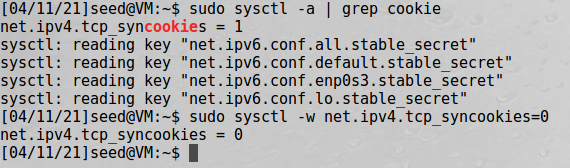
\includegraphics[scale=0.7]{1/9.png}\\\\
We notice that the attack was not successful when SYN cookie was turned on. The SYN cookie can effectively prevent the server from SYN flood attack because it does not allocate resources when it receives the SYN packet, it allocates resources only if the server receives the final ACK packet. This prevents from having the queue as a bottleneck, and instead consume resources only for the established connections.\\\\
SYN cookies also prevents an ACK flood attack by calculating an initial sequence number using a key known only to the server on certain parameters of the received SYN packet and sending it in SYN ACK packet. This sequence number + 1 is sent back in the ACK packet in the acknowledgment field. The server verifies the acknowledgement number and ensures that it was a result of a SYN ACK packet. This prevents any system from the SYN flood attacks.\\\\
\subsection{Task 2: TCP RST Attacks on telnet and ssh Connections}
\subsubsection{Using Netwox}
We first establish a \verb+telnet+ connection from the client 10.0.2.15 to the server 10.0.2.4:\\\\
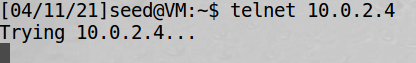
\includegraphics[scale=0.7]{1/10.png}\\\\
Now on the Attacker's VM we launch the RST attack.\\\\
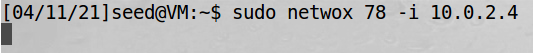
\includegraphics[scale=0.7]{1/11.png}\\\\
We can see that the connection between client and server was closed. The attack succeeded.\\\\
\pagebreak
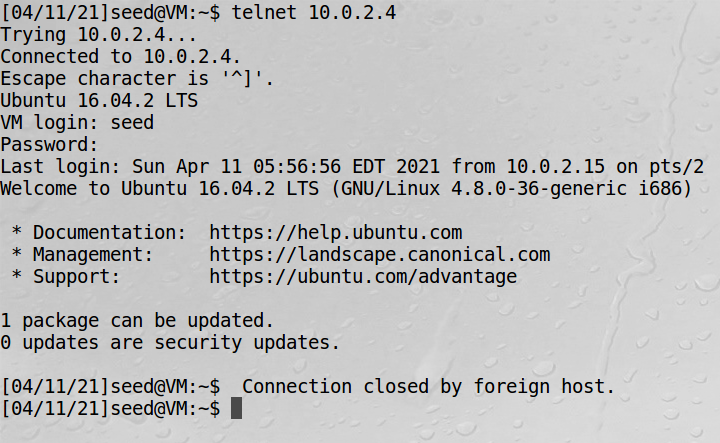
\includegraphics[scale=0.7]{1/12.png}
\\And it is the same with \verb+ssh+ connections:\\\\
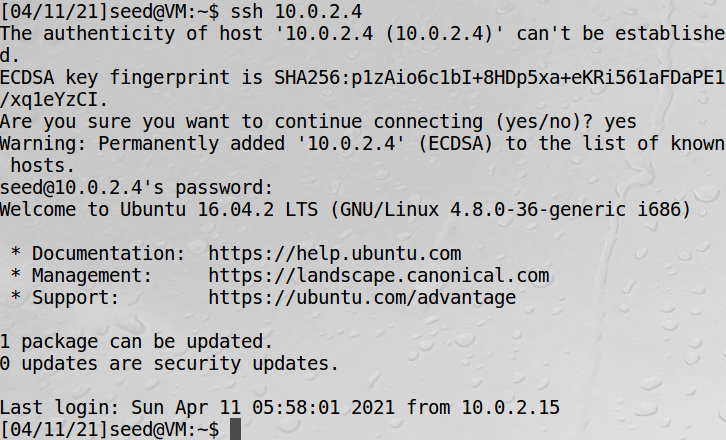
\includegraphics[scale=0.7]{1/13.png}\\\\
It breaks as soon as we launch an RST attack.\\\\
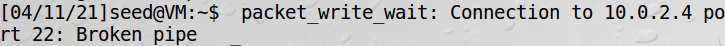
\includegraphics[scale=0.7]{1/14.png}\\\\
\subsubsection{Using Scapy}
We first establish a connection between the client and the server as shown below:\\\\
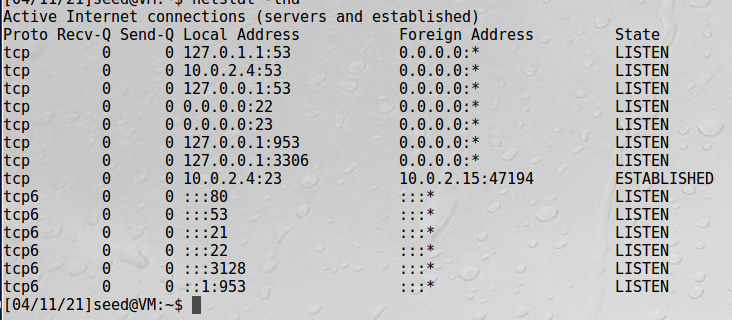
\includegraphics[scale=0.7]{1/15.png}\\\\
Then on the attacker's VM we check the latest TCP packet:\\\\
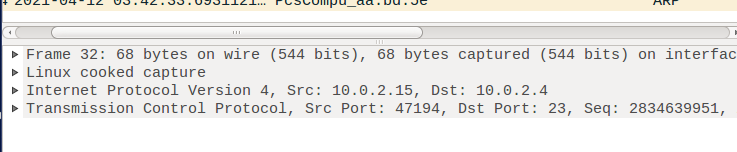
\includegraphics[scale=0.7]{1/16.png}\\\\
We obtained the ports, sequence and acknowledgement info from the packets, so now we craft the \verb+scapy+ script as follows:\\\\
\pagebreak

\includegraphics[scale=0.7]{1/17.png}
\\The attack is successful.\\\\
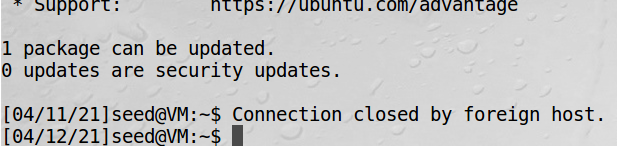
\includegraphics[scale=0.7]{1/18.png}\\\\
Let's try it again on an \verb+ssh+ connection. Again we use Wireshark to obtain info:\\\\
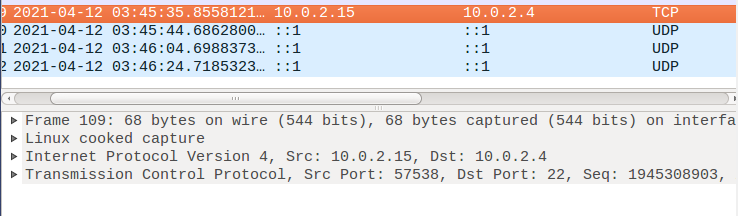
\includegraphics[scale=0.7]{1/19.png}\\\\
We then make the \verb+scapy+ script:\\\\
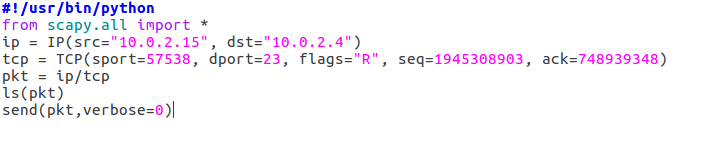
\includegraphics[scale=0.7]{1/20.png}\\\\
And the connection breaks again. The attack is successful.\\\\
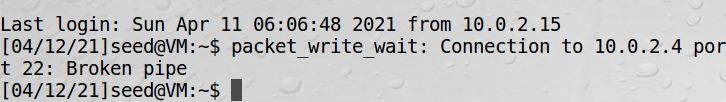
\includegraphics[scale=0.7]{1/21.png}\\\\
\subsection{Task 3: TCP Session Hijacking}
\subsubsection{Using Netwox}
Again we have a TCP connection established between the client and the server:\\\\
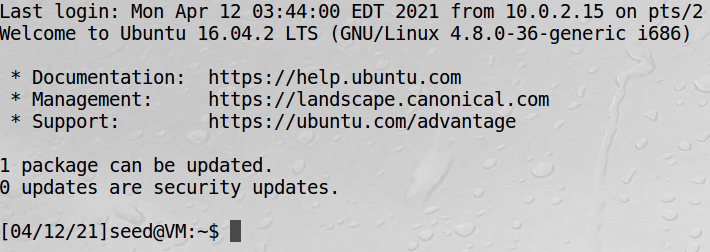
\includegraphics[scale=0.7]{1/22.png}\\\\
The aim of my attack is to create a text file on the victim's machine. We first convert the command to a hex string:\\\\
\pagebreak
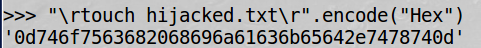
\includegraphics[scale=0.7]{1/23.png}
\\On Wireshark we check the latest TCP packet sent from the client to the server, and obtain various info.\\\\
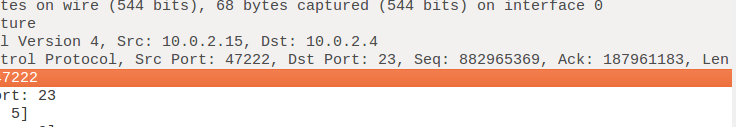
\includegraphics[scale=0.7]{1/24.png}\\\\
Then we can craft a packet using \verb+netwox+:\\\\
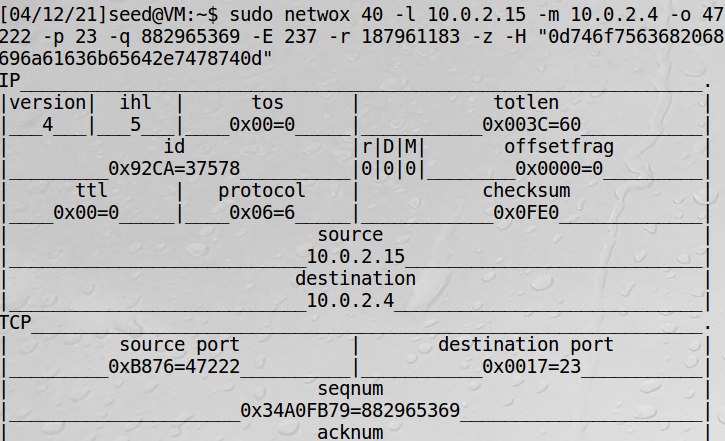
\includegraphics[scale=0.7]{1/25.png}\\\\
From Wireshark we can see that the command has been injected to the victim's VM and response was given.\\\\
\pagebreak
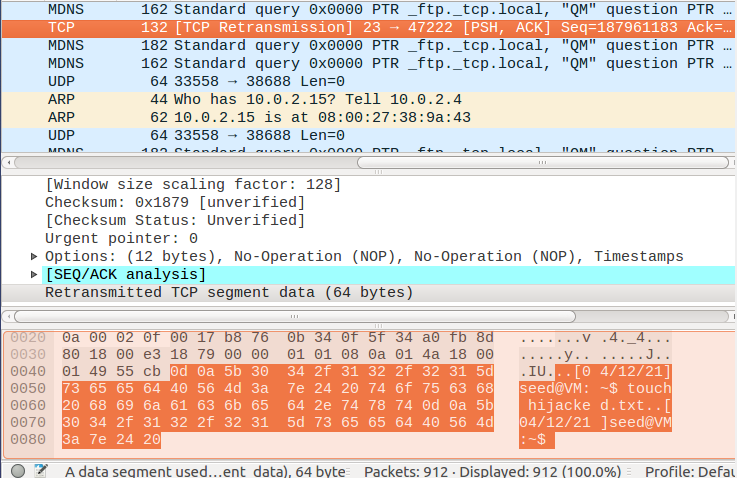
\includegraphics[scale=0.7]{1/26.png}
\\Here is the result. This indicates that we were able to hijack the session between the client and server and sent a command 
from the attacker’s machine in a way that it seemed to be coming from the client.\\\\
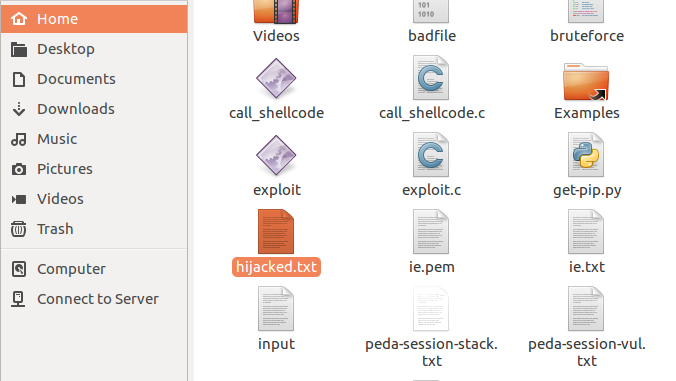
\includegraphics[scale=0.7]{1/27.png}\\\\
\subsubsection{Using Scapy}
Again we check the latest TCP packet sent from the client to the server, and obtain various info.\\\\
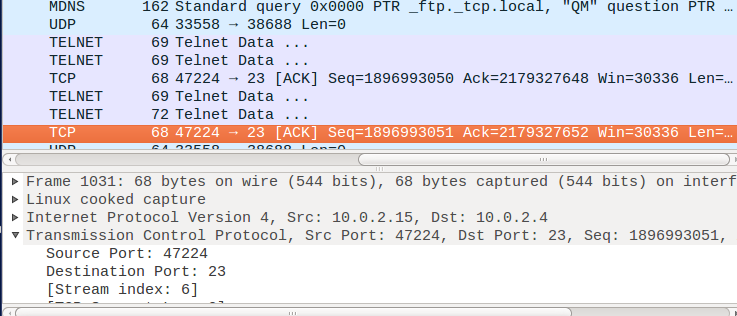
\includegraphics[scale=0.7]{1/28.png}\\\\
Then we craft the \verb+scapy+ script using the info:\\\\
\pagebreak
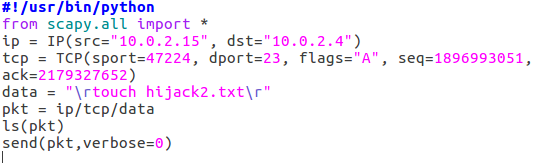
\includegraphics[scale=0.7]{1/29.png}
\\Now we execute the script.\\\\
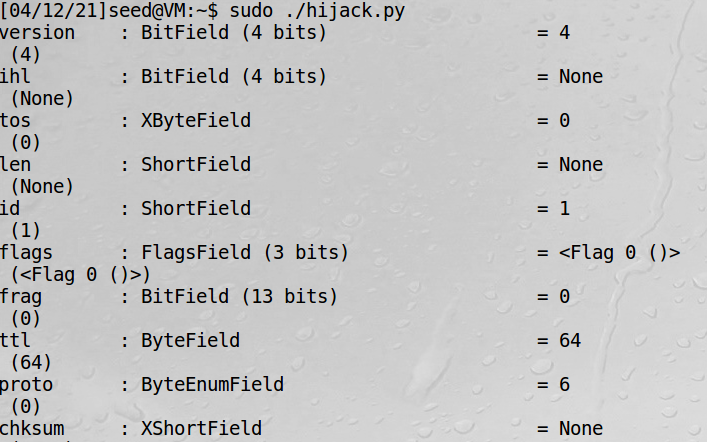
\includegraphics[scale=0.7]{1/30.png}\\\\
From Wireshark we can see that the command has been injected to the victim's VM and response was given.\\\\
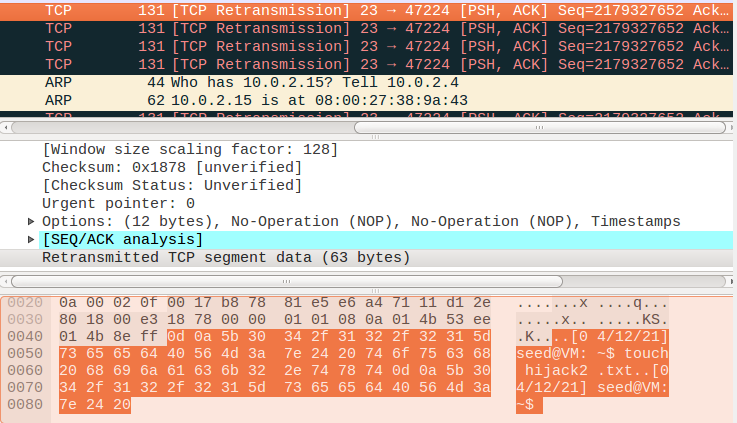
\includegraphics[scale=0.7]{1/31.png}\\\\
Again the attack is successful.\\\\
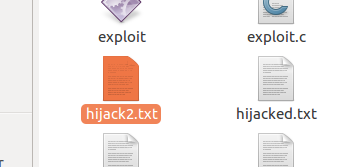
\includegraphics[scale=0.7]{1/32.png}\\\\
\pagebreak
\subsection{Task 4: Creating Reverse Shell using TCP Session Hijacking}
First we establish a \verb+telnet+ connection between the client and the server. We sniff the traffic and find the last packet sent from client to the server:\\\\
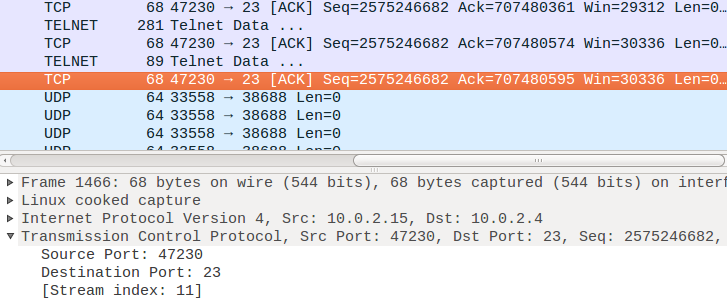
\includegraphics[scale=0.7]{1/33.png}\\\\
Following the guidelines we craft a \verb+scapy+ script that connects back to the attack's VM.\\\\
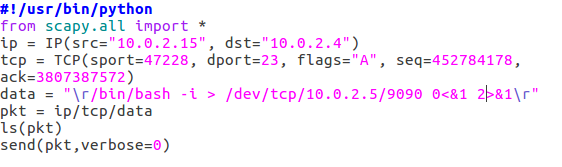
\includegraphics[scale=0.7]{1/34.png}\\\\
We then execute the script:\\\\
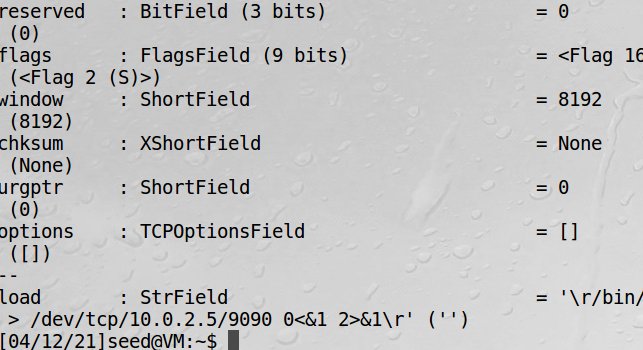
\includegraphics[scale=0.7]{1/35.png}\\\\
From Wireshark, we can see that the packet was sent and accepted by the server.\\\\
\pagebreak
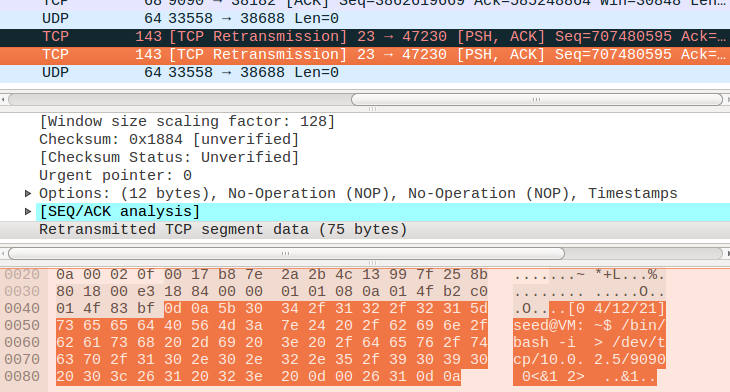
\includegraphics[scale=0.7]{1/36.png}\\
On the attacker's machine, while we were listening to port 9090, we are connected to the server directly when the script executes. We now have access to the victim's shell. Therefore, the attack is successful.\\\\
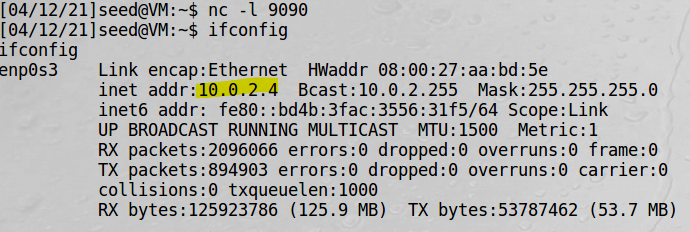
\includegraphics[scale=0.7]{1/37.png}
\pagebreak
\section{XSS Attack Lab}
\subsection{Task 5: Posting a Malicious Message to Display an Alert Window}
We let the attacker be Alice this time. We first write the provided JavaScript code into the "About me" field of Alice.\\
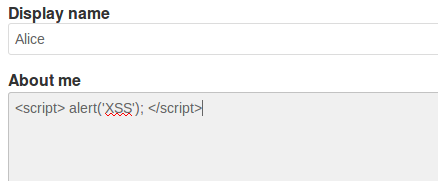
\includegraphics[scale=0.7]{2/1.png}\\\\
After saving the changes, the profile page loads again and display the pop up with the string "XSS", which we wrote in the code.\\
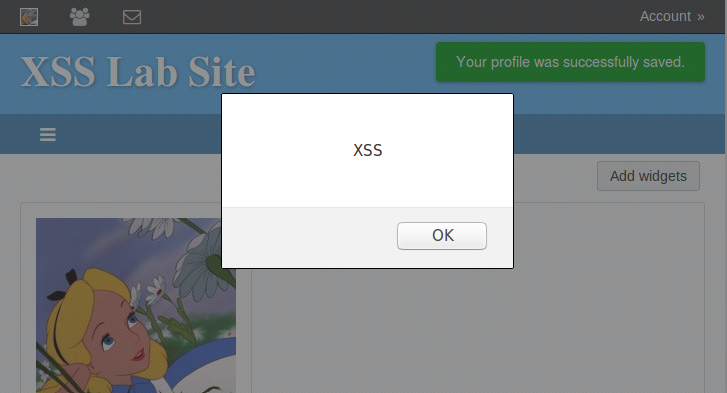
\includegraphics[scale=0.7]{2/2.png}\\\\
\subsection{Task 6: Posting a Malicious Message to Display Cookies}
Now we modify the code in Alice's profile as follows:\\
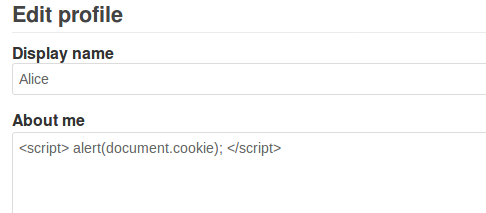
\includegraphics[scale=0.7]{2/3.png}\\\\
As the page reloads when we save the changes, we can immediately see that the cookie of the current session displays:\\
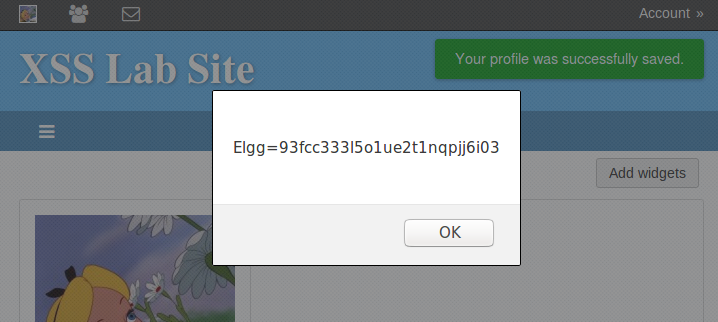
\includegraphics[scale=0.7]{2/4.png}\\\\
\subsection{Task 7: Stealing Cookies from the Victim’s Machine}
As an attacker, we first start a listening TCP connection in the terminal on the port 5555:\\
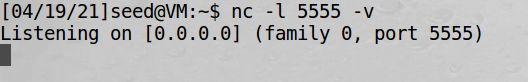
\includegraphics[scale=0.7]{2/5.png}\\\\
Now, in order to get the cookie of the victim, we insert the following JS code in the attacker's (Alice) description:\\
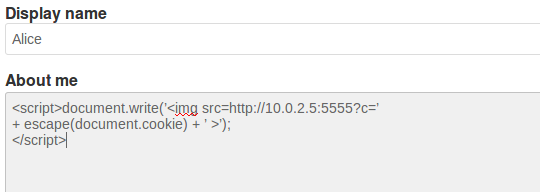
\includegraphics[scale=0.7]{2/6.png}\\\\
As soon as we save the changes, we can see Alice's HTTP request and cookie on the terminal:\\
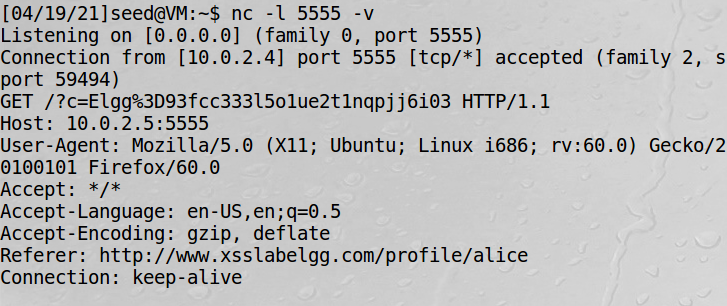
\includegraphics[scale=0.7]{2/7.png}\\\\
Now we start a new listening TCP connection, login as a victim Boby and visit Alice's profile page:\\
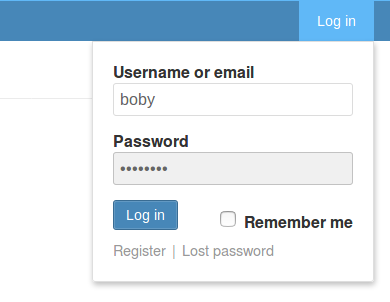
\includegraphics[scale=0.7]{2/8.png}\\\\
\pagebreak
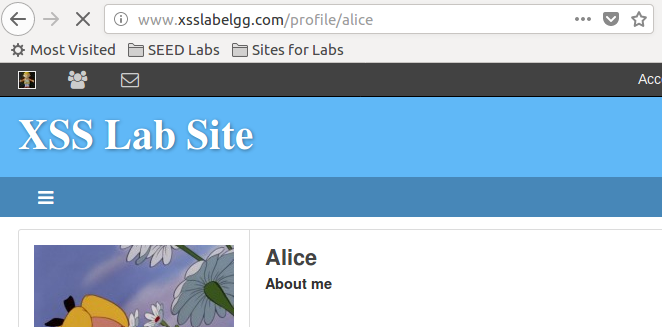
\includegraphics[scale=0.7]{2/9.png}\\\\
We can see that as soon as we visit Alice's page using Boby's account, we obtain the HTTP request indicating his cookie:\\
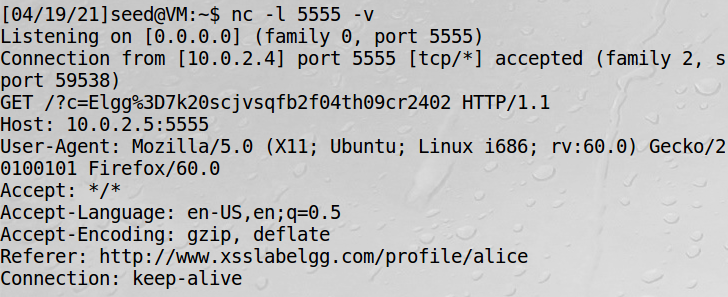
\includegraphics[scale=0.7]{2/10.png}\\\\
\subsection{Task 8: Becoming the Victim’s Friend}
In order to create a HTTP request that add Samy as a friend in other users' account, we need to figure out how the request works. Using Firefox's built in tools, we inspect the HTTP request made when we add Samy using Alice's account:\\
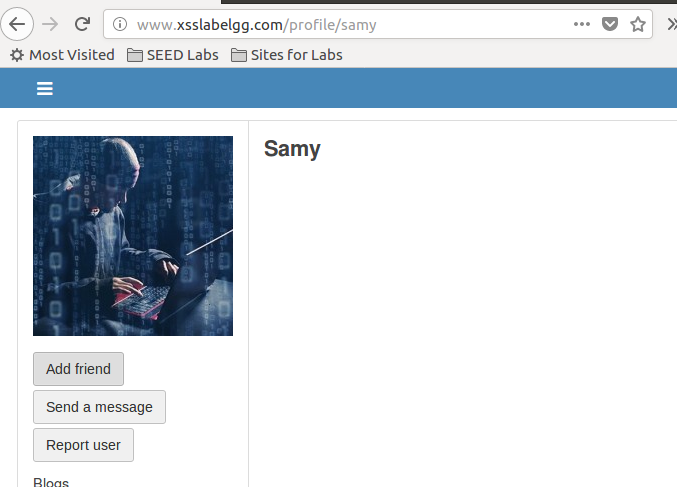
\includegraphics[scale=0.7]{2/11.png}\\\\
We can see that it's a GET request with a request URL:\\
\pagebreak
\includegraphics[scale=0.7]{2/12.png}\\\\
Now we look at the parameters we need:\\
\includegraphics[scale=0.7]{2/13.png}\\\\
These are the countermeasures implemented but we can get them from the JS variables. Now we add the code in Samy's profile that triggers the victim to send out the HTTP request we need:\\
\includegraphics[scale=0.7]{2/14.png}\\\\
\includegraphics[scale=0.7]{2/15.png}\\\\
As soon as we save the changes, the code is executed. The first thing we can notice is that Samy added himself! Of course it is the effect of the code, as on the website we have no other mean to do such operation.\\
\includegraphics[scale=0.7]{2/16.png}\\\\
Now we log into Boby's account and visit Samy's profile. Then we can see that he is now a friend with Samy without Boby's consent.\\
\includegraphics[scale=0.7]{2/17.png}\\\\
\pagebreak
\subsubsection{Question 1}
Line 1 and 2 represent the secret token and timestamp value attached to the HTTP request. They are defence mechanisms against untrusted cross-site request. The token is signed and the server verifies its authenticity and only then responds to the request. The timestamp indicates the time the request was sent. However, we can make use of them as they are saved as JS variables and stored in the AJAX variables that are used to construct the GET URL.
\subsubsection{Question 2}
No, we will not be able to launch the attack anymore. The editor mode encodes all special characters in the input, for example $<$ is replaced by \&lt. As we need at least the tag $<$script$>$ for a JS code to work, we will no longer have a code to be executed.
\subsection{Task 9: Modifying the Victim’s Profile}
To modify the victim's profile, we first need to see how a request is sent when we modify a profile. Using Samy's account, we try to modify the "About me" section:\\
\includegraphics[scale=0.7]{2/18.png}\\\\
We also monitor the network traffic when we save the changes. Then we can see the POST request sent:\\
\includegraphics[scale=0.7]{2/19.png}\\\\
Now we look at the params of the request:\\
\includegraphics[scale=0.7]{2/20.png}\\\\
We see that the description parameter represents the string we entered, and the access level 2 indicates its public visibility. Also, the guid is set as Samy's GUID. So, we now have enough information to construct a code that makes POST request:\\
\includegraphics[scale=0.7]{2/21.png}\\\\
We save the code in Samy's profile. Then, we log into Alice's account and go to Samy's profile and see the following:\\
\includegraphics[scale=0.7]{2/22.png}\\\\
The attack is successful, as we changed Alice's profile without her consent.\\
\subsubsection{Question 3}
We need Line 1 so that Samy does not accidentally attack himself as we reload his profile page. If we do not have that line, the code replaces itself we the string we intend to place on the victim's profile. There will not be any code left on Samy's profile to attack the victims.\\\\
Removing Line 1:\\
\pagebreak
\includegraphics[scale=0.7]{2/23.png}\\\\
As soon as we save the code, Samy's profile changes, and the attack became useless:\\
\includegraphics[scale=0.7]{2/24.png}\\\\
There is no JS code anymore and will not be any XSS attack.
\subsection{Task 10: Countermeasures}
For this task we add back Line 1 of the code.\\\\
First we activate the \verb+HTMLawed+ plugin on the elgg website:\\
\includegraphics[scale=0.7]{2/25.png}\\\\
We log into Alice's account and check Samy's profile. Now we see the following:\\
\pagebreak
\includegraphics[scale=0.7]{2/26.png}\\\\
We see that the plugin has displayed the entire code and it is not executed. This is because the plugin has converted the code into data. Now we turn on the \verb+htmlspecialchars+ countermeasure:\\
\includegraphics[scale=0.7]{2/27.png}\\\\
We can see that the result is similar. \verb+HTMLawed+ sanitized the HTML web page against XSS attack, and \verb+htmlspecialchars+ encoded the special characters into data. These two countermeasures made sure that the code is read as data by the browser and hence preventing XSS attack.
\includegraphics[scale=0.7]{2/28.png}\\\\
\end{document}